%manuel 6e, chapitre G3
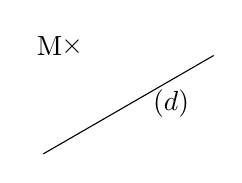
\begin{tikzpicture}[scale=0.5,every node/.style={scale=1},rotate=30]

\draw (0,2) node [left]{M};
\draw (0,2) node {$\times$};
\draw (-2,0)--(3,0) node [near end,below] {$(d)$};


\end{tikzpicture} 
